\soustitre{Énoncés}


\begin{exo}
	Déterminer tous les entiers positifs $x$, $y$ et $z$ tels que
	\[x^2+ y^2 - 15 = 2^z.\]
\end{exo}



\begin{exo}
	On se donne un ensemble $S$ de $n \geq 5$ points du plan, coloriés en rouge et noir.
	On suppose que trois points de la même couleur ne sont jamais alignés. 
	
	Montrer que l'on peut trouver trois points de la même couleur formant un triangle dont au moins l'un des côtés ne contient pas de point de $S$.
\end{exo}

\begin{exo}{}
	Déterminer les entiers positifs $x$ et $y$ tels que
	\[\left( 1 + \frac{1}{x}\right) \left(1 + \frac{1}{y} \right) = \frac{3}{2}.\]
\end{exo}


\begin{exo}
	Un pion est placé sur un échiquier $6\times6$. Il peut se déplacer horizontalement ou verticalement en sautant d'une case, puis de deux, puis d'une, puis de deux $\ldots$
	
	Déterminer s'il est possible de choisir une case initiale pour le pion de façon à ce qu'il puisse passer par toutes les cases de l'échiquier par une suite de 35 sauts respectant cette alternance.
\end{exo}

\soustitre{Solutions}

\bigskip

\begin{sol}
	Comme un carré est congru à $0$ ou $1$ modulo $4$ on a 
	\[\begin{aligned}
		x^2 & \equiv 0 \text{ ou } 1 &\mod 4 \\
		y^2 & \equiv 0 \text{ ou } 1 &\mod 4 \\
		-15 & \equiv 1 \text{ ou } 1 &\mod 4 \\
	\end{aligned}\]
	et par conséquent 
	\[x^2 + y^2 - 15 \equiv 1, 2 \text{ ou } 3 \mod 4.\]

	Or si $z \geq 2$ on a $2^z \mod 0 \mod 4$.

	Par conséquent il n'y a pas de solution si $z \geq 2$.

	Il suffit ensuite de traiter les cas $z=0$ et $z=1$.


	\begin{itemize}
		\item Si $z=0$, on obtient l'équation
		\[x^2 + y^2 = 16.\]

		Comme un carré est toujours positif on a en particulier 
		\[x^2 \leq 16\]
		et par positivité de $x$ il suffit de traiter les cas $0 \leq x \leq 4$.

		\begin{itemize}
			\item Pour $x = 0$, l'équation
			\[0^2 + y^2 = 16\]
			admet $y = 4$ comme solution.
			\item Pour $x = 1$, l'équation
			\[1^2 + y^2 = 16\]
			n'admet pas de solution entière.
			\item Pour $x = 2$, l'équation
			\[2^2 + y^2 = 16\]
			n'admet pas de solution entière.
			\item Pour $x = 3$, l'équation
			\[3^2 + y^2 = 16\]
			n'admet pas de solution entière.
			\item Pour $x = 4$, l'équation
			\[4^2 + y^2 = 16\]
			admet $y = 0$ comme solution.
		\end{itemize}
		
		\item Si $z=1$, on obtient l'équation
		\[x^2 + y^2 = 19.\]

		Comme un carré est toujours positif on a en particulier 
		\[x^2 \leq 19 < 25\]
		et par positivité de $x$ il suffit de traiter les cas $0 \leq x \leq 4$.

		\begin{itemize}
			\item Pour $x = 0$, l'équation
			\[0^2 + y^2 = 17\]
			n'admet pas de solution.
			\item Pour $x = 1$, l'équation
			\[1^2 + y^2 = 17\]
			admet $y=4$ comme solution.
			\item Pour $x = 2$, l'équation
			\[2^2 + y^2 = 17\]
			n'admet pas de solution entière.
			\item Pour $x = 3$, l'équation
			\[3^2 + y^2 = 17\]
			n'admet pas de solution entière.
			\item Pour $x = 4$, l'équation
			\[4^2 + y^2 = 17\]
			admet $y = 1$ comme solution.
		\end{itemize}
		\end{itemize}

		Par conséquent l'ensemble des solutions est

		\[\boxed{\left\lbrace (0,4,0),(4,0,0),(4,1,1),(1,4,1)\right\rbrace}.\]


		\underline{Remarque}: il aurait été possible de réduire le nombre de cas à vérifier en remarquant que, par symétrie du problème, quitte à intervertir $x$ et $y$ on peut supposer $x \leq y$.

\end{sol}

\begin{sol}
	Puisque $n$ vaut au moins $5$, par \emph{principe des tiroirs} il y a $3$ points de la même couleur formant un triangle.
	
	
	Montrons qu'un triangle de périmètre \emph{minimal} parmi tous les triangles monochromatiques convient.

	Supposons par l'absurde que les $3$ côtés d'un tel triangle de périmètre minimal contiennent des point de $S$. Comme $3$ points de la même couleur ne sont jamais alignés, ces $3$ points sont tous de couleur différente que celle des sommets du triangle. Ils forment donc un triangle monochromatique de plus petit périmètre. Contradiction.
\end{sol}

\begin{sol}
	L'idée est de majorer $x$ et $y$ pour se ramener à un nombre fini de cas à tester.

	On commence par remarquer que, par \emph{symétrie du problème} et quitte à intervertir $x$ et $y$, on peut supposer que $x \leq y$.

	Par conséquent comme
	\[0 < x \leq y\]
	on obtient
	\[0 < \frac{1}{y} \leq \frac{1}{x}\]
	donc
	\[0 < 1+\frac{1}{y} \leq 1+\frac{1}{x}\]
	et donc
	\[\left(1 + \frac{1}{x} \right)^2 \geq \left( 1 + \frac{1}{x}\right) \left(1 + \frac{1}{y} \right) = \frac{3}{2}.\]

	Par croissance de la racine sur les réels positifs on obtient
	\[1 + \frac{1}{x} \geq \sqrt{\frac{3}{2}}\]
	donc
	\[\frac{1}{x} \geq \sqrt{\frac{3}{2}}-1 > 0\]
	et donc
	\[0 < x \leq \frac{1}{\sqrt{\frac{3}{2}}-1}.\]


	Il reste à estimer cette borne. On peut par exemple remarquer que $\left( \frac{6}{5}\right)^2 = \frac{36}{25} < \frac{3}{2}$.

	Par conséquent $\sqrt{\frac{3}{2}} > \frac{6}{5}$
	\[0 < x < \frac{1}{\frac{6}{5}-1} = 5.\]

	Il suffit donc de regarder pour $x =1, 2, 3 \text{ ou } 4$.

	\begin{itemize}
		\item Pour $x=1$ on obtient comme équation
		\[\left(1 + \frac{1}{1} \right)\left(1 + \frac{1}{y} \right) = \frac{3}{2}\]
		c'est à dire
		\[\frac{1}{y} = -\frac{1}{4}\]
		qui n'admet pas de solution entière.
		\item Pour $x=2$ on obtient comme équation
		\[\left(1 + \frac{1}{2} \right)\left(1 + \frac{1}{y} \right) = \frac{3}{2}\]
		c'est à dire
		\[\frac{1}{y} = 1\]
		qui n'admet pas de solution entière.
		\item Pour $x=3$ on obtient comme équation
		\[\left(1 + \frac{1}{3} \right)\left(1 + \frac{1}{y} \right) = \frac{3}{2}\]
		c'est à dire
		\[\frac{1}{y} = \frac{1}{8}\]
		de solution $y=8$.
		\item Pour $x=4$ on obtient comme équation
		\[\left(1 + \frac{1}{4} \right)\left(1 + \frac{1}{y} \right) = \frac{3}{2}\]
		c'est à dire
		\[\frac{1}{y} = \frac{1}{5}\]
		de solution $y=5$.
	\end{itemize}

	Par symétrie l'ensemble des solutions est donc
	\[\boxed{\left\lbrace (3,8), (4,5), (8,3), (5,4) \right\rbrace}.\]
\end{sol}

\begin{sol}
	Nous allons montrer qu'une telle case n'existe pas.

	\underline{Méthode 1} : On colorie l'échiquier en trois couleurs, bleu, blanc et rose, comme ci-dessous.
	\begin{center}
		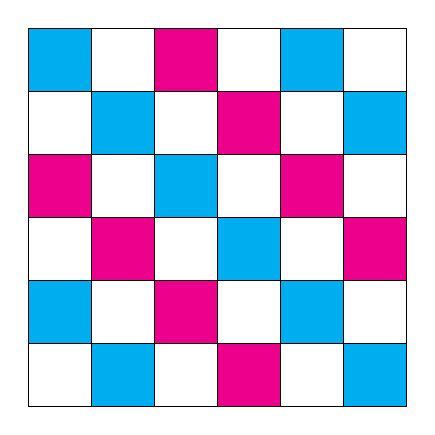
\begin{tikzpicture}[scale=0.8]
		\draw (0,0) grid (6,6);
		\foreach \i in {0,...,5}{
				\pgfmathtruncatemacro{\j}{5-\i}
				\draw [fill=cyan] (\i,\j)--(\i,\j+1)--(\i+1,\j+1)--(\i+1,\j)--(\i,\j);
			}
		\foreach \i in {0,...,1}{
				\pgfmathtruncatemacro{\j}{1-\i}
				\draw [fill=cyan] (\i,\j)--(\i,\j+1)--(\i+1,\j+1)--(\i+1,\j)--(\i,\j);
			}
		\foreach \i in {0,...,1}{
				\pgfmathtruncatemacro{\j}{1-\i}
				\draw [fill=cyan] (5-\i,5-\j)--(5-\i,5-\j+1)--(5-\i+1,5-\j+1)--(5-\i+1,5-\j)--(5-\i,5-\j);
			}
		\foreach \i in {0,...,3}{
				\pgfmathtruncatemacro{\j}{3-\i}
				\draw [fill=magenta] (\i,\j)--(\i,\j+1)--(\i+1,\j+1)--(\i+1,\j)--(\i,\j);
			}
		\foreach \i in {0,...,3}{
				\pgfmathtruncatemacro{\j}{3-\i}
				\draw [fill=magenta] (5-\i,5-\j)--(5-\i,5-\j+1)--(5-\i+1,5-\j+1)--(5-\i+1,5-\j)--(5-\i,5-\j);
			}
	\end{tikzpicture}
	\end{center}
	

	Supposons que la case initiale cherchée existe.


	Quitte à passer au coloriage symétrique, on peut supposer que cette case est blanche. Examinons alors le déroulement d'un parcours de $35$ sauts. On commence sur une case blanche, puis on fait un saut d'une case, vers une case non-blanche donc. Le saut suivant, de deux cases, nous amène vers une case de l'autre couleur non-blanche. Les sauts d'une case, puis de deux cases suivants nous amènent alors sur une case blanche. On est alors revenu à la situation de départ : sur une case blanche avec un saut d'une case à faire. On répète alors ce processus huit fois (sauf le dernier saut de deux cases la dernière fois).

	Ainsi, les cases roses et bleues vont par paires ; à toute case bleue on peut associer une case rose qui est visitée juste avant ou juste après dans le parcours. 
	
	Comme il y a huit cases roses et dix cases bleues, c'est la contradiction cherchée.


	\medskip

	\underline{Méthode 2} : on colorie l'échiquier en deux couleurs :
	\begin{center}
		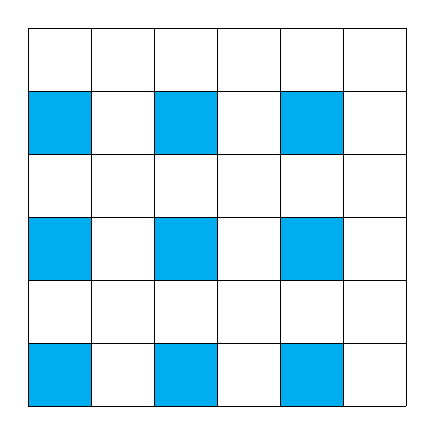
\begin{tikzpicture}[scale=0.8]
		\draw (0,0) grid (6,6);
		\foreach \i in {0,...,2}{
				\foreach \j in {0,...,2}{
						\draw [fill=cyan] (2*\i,2*\j)--(2*\i,2*\j+1)--(2*\i+1,2*\j+1)--(2*\i+1,2*\j)--(2*\i,2*\j);
					}
			}
	\end{tikzpicture}
	\end{center}
	

	Un saut de deux cases partant d'une case bleue ne peut arriver que sur une autre case bleue. Dès lors, à toute case bleue on peut associer une autre case bleue qui lui est adjacente dans le parcours, sauf si cette case est la case de départ ou d'arrivée. Pour éviter une contradiction, il faut donc que la case de départ ou d'arrivée soit bleue (puisqu'on a un nombre impair de case bleues).
	
	Comme on peut refaire le même raisonnement en décalant les cases bleues vers le haut ou vers la droite, on est forcé d'avoir au moins trois cases bleues qui sont de départ ou d'arrivée, ce qui est une contradiction.


\end{sol}